\chapter{Using \sysname{} to provide a \commonlisp{} reader}

\sysname{} can be used to provide the reader of a \commonlisp{}
implementation.

\section{Using}

\texttt{cl:peek-char}
\texttt{cl:read-char}
\texttt{cl:unread-char}
\texttt{cl:with-input-from-string}

\begin{figure}
  \centering
  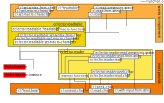
\includegraphics[angle=90]{figures/reader-implementation.pdf}
  \caption{Implemenation}
  \label{fig:reader-implementation}
\end{figure}

\newpage{}

\begin{sidewaystable}
  \begin{tabular}{l|p{.08\linewidth}|p{0.25\linewidth}|p{0.25\linewidth}}
    Function                               & Host provides & \sysname{} provides                         & Why \\
    \hline
    \texttt{cl:peek-char}                  & must          & \texttt{e.r:peek-char}                      & Peek based on \sysname{}'s readtable\\
    \texttt{cl:read-char}                  & must          & \texttt{e.r:read-char}                      & \sysname{}'s \texttt{end-of-file}\\
    \texttt{cl:unread-char}                & must          & no                                          & \\
    \hline
    \texttt{cl:read}                       & may           & \texttt{eclector.reader:read}               & \\
                                           &               & \texttt{e.p-r:read}                         & custom parse result \\
                                           &               & \texttt{e.c-s-t:read}                       & convenience \\
    \texttt{cl:read-preserving-whitespace} & may           & \texttt{e.r:read-preserving-whitespace}     & \\
                                           &               & \texttt{e.p-r:read-preserving-whitespace}   & custom parse result \\
                                           &               & \texttt{e.c-s-t:read-preserving-whitespace} & convenience \\
    \texttt{cl:read-from-string}           & may           & \texttt{e.r:read-from-string}               & \\
                                           &               & \texttt{e.p-r:read-from-string}             & custom parse result \\
                                           &               & \texttt{e.c-s-t:read-from-string}           & convenience \\
                                                                                                     & \\
    \hline
    \texttt{cl:with-input-from-string}     & must          & no                                      & \\
  \end{tabular}
\end{sidewaystable}

\inputcode{../examples/eclector-as-implementation-reader.code}